\documentclass[]{beamer}
% \geometry{papersize={16cm,9.60cm}}
\usepackage{etex}
\usepackage{amsmath}
\usepackage{tikz}
\usepackage{multimedia}
\usetheme{Boadilla}
\usepackage{graphicx}
\usepackage{url}

%\usepackage{inputenc}

% \mode<presentation>
% {
%   \usetheme{default}
%   \setbeamercovered{transparent}
% }


% {\vskip5pt}

%% customize layout, bullet points navigation toolbar
\setbeamertemplate{navigation symbols}{}%remove navigation symbols
\setbeamertemplate{enumerate items}[default]
\setbeamertemplate{navigation symbols}{}
\setbeamertemplate{itemize items}[circle]
\setbeamercolor{enumerate item}{fg=black}

\setbeamertemplate{footline}{}
\setbeamersize{text margin left = 2.0em}
\setbeamersize{text margin right = 2.0em}


\usepackage{times}
\usepackage[T1]{fontenc}

% Or whatever. Note that the encoding and the font should match. If T1
% does not look nice, try deleting the line with the fontenc.

\setbeamertemplate{navigation symbols}{}

\title{ Cognitive (Neuro) Psychology }
\subtitle{X. Memory, Learning and Forgetting}
\author{ Marianne Maertens }
\institute[TU Berlin]{Technische Universit\"at Berlin}
\date{September 2016}

\begin{document}
\setbeamertemplate{enumerate items}[default]
\setbeamertemplate{headline}

\frame{\titlepage}

\AtBeginSection[]
{
  \begin{frame}<beamer>
    \frametitle{Layout}
    \tableofcontents[currentsection]
  \end{frame}
}

\begin{frame}
 \frametitle{Memory}
\begin{overlayarea}{130mm}{70mm}


\begin{columns}[T]
 \begin{column}{50mm}
\begin{center}
\begin{itemize}
 \item<1-> what is familiar
 \item<2-> talk, read, write
 \item<3-> sense of time and space
 \item<3-> sense of self
 \item<4-> culture
 \item<5->defines \textbf{personality}
\end{itemize}
\end{center}
 \end{column}
 \begin{column}{70mm}
\vspace{5mm}
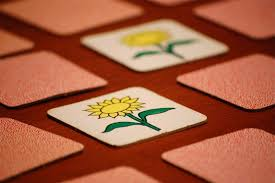
\includegraphics[width=50mm]{figs/l10/memory_game.jpg}
 \end{column}
\end{columns}
\end{overlayarea}
 \end{frame}


\begin{frame}
\frametitle{Memory}
 \begin{overlayarea}{110mm}{70mm}

\begin{itemize}
 \item architecture vs. processes of memory
 \begin{itemize}
 \item architecture: short-term vs long-term
 \item processes: 
 \end{itemize}
\end{itemize}

 \begin{center}
\includegraphics<2>[width=100mm]{figs/l10/memory_retrieval.png}
 \end{center}
\end{overlayarea}
\end{frame}


\begin{frame}
 \frametitle{Outline}
\begin{itemize}[<+->]
  \setlength{\itemsep}{5pt}
 \item Architecture
 \item Working memory
 \item Working memory \& other cognitive functions
%  \item Levels of processing
 \item Learning through retrieval
 \item Implicit learning
 \item Forgetting
\end{itemize}
\end{frame}


\begin{frame}
 \frametitle{Architecture: Multi-store model}
\begin{overlayarea}{110mm}{80mm}

\begin{center}
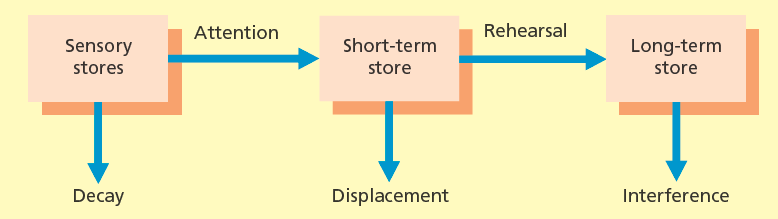
\includegraphics[width=90mm]{figs/l10/multi_store_model.png}

Atkinson and Shiffrin, 1968
\end{center}
\only<2>{
\textbf{Sensory stores}
 \begin{itemize}
 \item Iconic memory - lasts 500ms to 1.6sec
 \item Echoic memory - lasts up to 2.4sec - ``playback'' facility
 \end{itemize}
}
\only<3>{
\textbf{Short-term memory (STM)}
 \begin{itemize}
 \item limit:
 \begin{itemize}
 \item digit span of approx 7 $\pm$2 items (Miller, 1956)
 \item ``chunks'' up to 4 (Cowan, 2000) 
 \item[] TNTIBMUFO vs TNT IBM UFO
 \end{itemize}
 \item loss of information: 
 \begin{itemize}
 \item decay $\rightarrow$ rehearsal
 \item interference $\rightarrow$ spacing
\end{itemize}
\end{itemize}
}
\only<4>{
\textbf{Long-term memory (LTM)}
 \begin{itemize}
 \item unlimited capacity
 \item information loss due to brain damage or time/age
 \end{itemize}
}
\end{overlayarea}
\end{frame}


\begin{frame}
 \frametitle{Iconic memory}
\begin{overlayarea}{120mm}{70mm}
 \textbf{ Partial report paradigm} (Sperling, 1960)
\begin{columns}[T]
 \begin{column}{30mm}
 \begin{center}
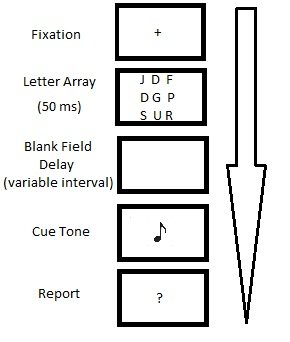
\includegraphics[width=50mm]{figs/l10/sperling_partial_report.jpg}
 \end{center}
 \end{column}

 \begin{column}{70mm}
\begin{itemize}
 \item[] whole report: 
 \item[] recall as many elements as possible 
 \item[] $\rightarrow$ 3-5 characters/12
 \item<2->[] cued report:
 \item<2->[] frequency of tone indicates which row to report
 \item<2->[] $\rightarrow$ 9-12 characters/12
 \item[]
 \item<3->[] variation of cue interval revealed survival time of about 1sec
\end{itemize}
 \end{column}
\end{columns}
\end{overlayarea}
\end{frame}


\begin{frame}
 \frametitle{Multi-store vs. unitary store models}
\begin{overlayarea}{120mm}{90mm}
\begin{itemize}
 \item differences vs. similarities between short- and long-term memory
 \item multi-store models: hippocampus and medial temporal lobes (damaged in amnesic patients) more involved in long- than in short-term memory
\end{itemize}

\only<2>{
\begin{columns}[T]
 \begin{column}{45mm}
\vspace{3mm}
 Race et al., 2013: 
\begin{itemize}
 \item Face recognition memory task
 \item Hippocampus damage alone - memory intact
\end{itemize}
 \end{column}

 \begin{column}{70mm}

\includegraphics<2->[width=60mm]{figs/l10/race13_face_recognition.png}
 \end{column}
\end{columns}
}
\end{overlayarea}
\end{frame}


\begin{frame}
 \frametitle{Short-term memory - STM}
\begin{center}
 Is short-term memory at all relevant?
\end{center}
\begin{itemize}
 \item<2-> allows us to retain a phone number for the few secs to dial it
 \item<3-> irrelevant as most people have mobile phones
\end{itemize}
\end{frame}

\begin{frame}
\begin{overlayarea}{110mm}{80mm}

Baddeley and Hitch, 1974
\begin{itemize}
 \item we use short-term memory to perform complex tasks e.g. mental arithmetic  
 \item STM relevant for numerous non-memory tasks
 \item<2->[$\Rightarrow$]  Short-term memory $\rightarrow$ \textbf{Working memory}
\end{itemize}
\only<3->{
 \begin{columns}[T]
 \begin{column}{35mm}
 \begin{center}
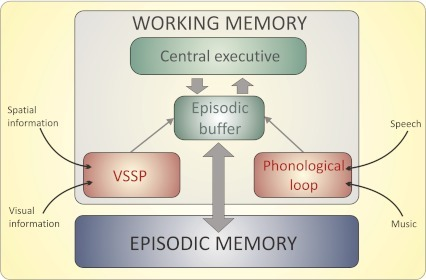
\includegraphics[width=40mm]{figs/l10/WM_architecture_2.png}
 \end{center}
 \end{column}

 \begin{column}{80mm}
\begin{itemize}
 \item central executive - ``attentional system''
 \item phonological loop - speech-based information
 \item visuo-spatial sketchpad - visual processing
 \item episodic buffer - temporary storage for integrated info from VSSP and PL 
\end{itemize}
 \end{column}
\end{columns}
}
\vspace{3mm}
\begin{itemize}
 \item<4->[!] limited capacity, independent of each other
 \item<4->[$\rightarrow$] if two tasks use the same component they cannot be performed together
\end{itemize}

\end{overlayarea}
\end{frame}



\begin{frame}
 \frametitle{Dual task performance}
\begin{overlayarea}{110mm}{80mm}
Robbins et al., 1996
\begin{itemize}
 \item selection of chess moves by weaker and stronger players
 \begin{itemize}
  \item repetitive tapping: control
  \item random number generation: central executive
  \item pressing keys on keypad in clockwise fashion: visuo-spatial sketchpad
  \item rapid repetition of word ``see-saw'': articulatory suppression using phonological loop

 \end{itemize}
\end{itemize}

 \begin{center}
\includegraphics<2->[width=60mm]{figs/l10/chess_robbins96.png}
 \end{center}
\end{overlayarea}
\end{frame}


\begin{frame}
 \frametitle{Phonological loop}
\begin{overlayarea}{110mm}{80mm}
 \begin{center}
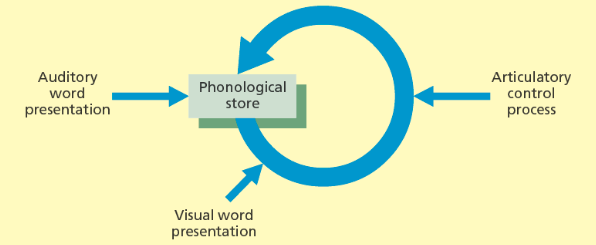
\includegraphics[width=60mm]{figs/l10/phonological_loop.png}
 \end{center}

\begin{itemize}
 \item passive phonological store concerned with speech perception
 \item articulatory process linked to speech production (rehearsal)
\end{itemize}
\only<2->{
Exeriment on memory span:
 \begin{itemize}
 \item Series of words is presented \textit{visually} and subjects are asked to immediately  recall the words in the correct order 
 \item[$\Rightarrow$] Would people use the phonological loop to engage in verbal rehearsal?
 \end{itemize}
}

\end{overlayarea}
\end{frame}

\begin{frame}
 \frametitle{Phonological similarity effect}
\begin{overlayarea}{120mm}{80mm}
Larsen et al., 2000 
\begin{columns}[T]
 \begin{column}{20mm}
 \begin{itemize}
  \item[] FEE 
  \item[] HE 
  \item[] KNEE 
  \item[] LEE 
  \item[] MEE 
  \item[] SHE 
 \end{itemize}
 \end{column}

 \begin{column}{20mm}
 \begin{itemize}
  \item[] BAY 
  \item[] HOE
  \item[] IT 
  \item[] ODD 
  \item[] SHY 
  \item[] UP 
 \end{itemize} 
 \end{column}
\end{columns}

\begin{itemize}
 \item<2->[$\Rightarrow$] immediate serial recall was 25\% worse with the phonologically similar list
 \item<3-> [BUT] not clear whether phonological similarity effect depends more on \textit{acoustic} similarity or on \textit{articulatory} similarity  
 \item<4->[!] significant effect of articulatory similarity when recall was \textit{spoken} but not when it was \textit{written}
\end{itemize}
\end{overlayarea}
\end{frame}


\begin{frame}
 \frametitle{Word length effect}
\begin{overlayarea}{120mm}{80mm}
 
\begin{itemize}
 \item[=] \textbf{word span} is greater for short than for long words
 \item[] (\# words recalled immediately in the correct order)
\end{itemize}

\only<2->{
Baddeley, 1974:
\begin{itemize}
 \item word length effect for visually and auditorily presented words
 \item articulatory suppression condition: repeat digits from 1 to 8 to prevent rehearsal within the phonological loop
 \item[$\Rightarrow$] no word-length effect with visually presented words 
\end{itemize}
}

\only<3->{
Jalbert et al., 2011:
\begin{itemize}
 \item[!] confound: word length correlates with \textbf{orthographic neighbourhood}
 \item[] (\# words of the same lenght differing in only one letter)
 \item<4-> word-length effect disappeared when short and long words were equated for orthographic neighbourhood size   
\end{itemize}
}
\end{overlayarea}
\end{frame}


\begin{frame}
 \frametitle{Phonological loop in the real world}
\begin{overlayarea}{120mm}{80mm}
\begin{itemize}
 \item[$\Rightarrow$] important for learning a foreign language
 \item[$\Rightarrow$] used for action control - ``inner voice''
\end{itemize}

 \begin{center}
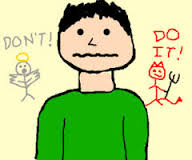
\includegraphics[width=60mm]{figs/l10/action_control.jpg}
 \end{center}
\end{overlayarea}
\end{frame}



\begin{frame}
 \frametitle{Central executive}
\begin{overlayarea}{110mm}{80mm}
\begin{itemize}
 \item most important and versatile component of working memory
 \item heavily involved in almost all complex cognitive activities but does not store information
 \item prefrontal cortex is the brain region \textit{most} involved in executive functions:
 \item[] repetitive TMS of dorsolateral prefrontal cortex impaired performance in many complex tasks
\end{itemize}

\only<2->{
Baddeley, 1996: Executive processes
\begin{enumerate}
 \item focusing attention
 \item dividing attention between stimuli
 \item switching attention between tasks 
 \item interfacing with long-term memory
\end{enumerate}
}
\begin{itemize}
 \item<3-> empirically difficult to obtain consensus on the number and nature of executive processes 
\end{itemize}
\end{overlayarea}
\end{frame}



\begin{frame}
 \frametitle{Number and nature of executive functions}
\begin{overlayarea}{110mm}{80mm}
Miyaki et al., 2000
\begin{itemize}
 \item participants were tested with several executive tasks
 \item use (positive) correlations among tasks to identify executive processes common to all tasks and unique for certain tasks
\end{itemize}


\begin{columns}[T]
 \begin{column}{60mm}
\begin{enumerate}
 \item<2-> \textit{Inhibition function} - override dominant responses, resist distraction 
 \item<3-> \textit{Shifting function} - switch flexibly between tasks or mental sets 
 \item<4-> \textit{Updating function} - monitor rapid addition or deletion of WM contents 
\end{enumerate}
 \end{column}

 \begin{column}{50mm}
 \includegraphics<2>[width=50mm]{figs/l10/stroop.png}
\begin{center}
 \includegraphics<3->[width=20mm]{figs/l10/task_switch.png}
\end{center}

 \end{column}
\end{columns}
\end{overlayarea}
\end{frame}

\begin{frame}
 \frametitle{Dysexecutive syndrome}
\begin{overlayarea}{110mm}{80mm}
 \begin{itemize}
  \item study brain-damaged individuals whose central executive functioning is impaired
  \item cognitive problems: impaired response inhibition, rule deduction and generation, maintenance and shifting of sets
 \end{itemize}
\only<2>{
\begin{exampleblock}{Demo: Wisconsin Card Sorting Test (WCST)}
 Go to the following website and run the WCST on yourself \url{http://www.psytoolkit.org/experiment-library/experiment_wcst.html}
\end{exampleblock}
}

\only<3->{
Stuss \& Alexander, 2007
\begin{itemize}
 \item testing patients with limited damage within prefrontal cortex they identified three executive processes:  
\end{itemize}
\begin{enumerate}
 \item \textit{Task setting} - set a stimulus-response relationship e.g. drive a car 
 \item \textit{Monitoring} - check adequacy on one's performance
 \item \textit{Energisation} - sustained attention or concentration
\end{enumerate}
}

\end{overlayarea}
\end{frame}



\begin{frame}
 \frametitle{Working memory capacity}
\begin{overlayarea}{110mm}{70mm}
\begin{itemize}
 \item individual differences in WM capacity
 \item WM capacity: amount of information an individual can process and store at the same time
\end{itemize}

\only<2>{
Daneman \& Carpenter, 1980: \textbf{Reading span}

\begin{itemize}
 \item read sentences for comprehension - \textit{processing task}
 \item recall the final word of each sentence - \textit{storage task}
 \item reading span = largest \# sentences from which individuals remember the final words more than 50\% of the time
 \item<3> high-capacity individuals need fewer WM resources to comprehend the sentences and hence have more capacity available to retain the last word
\end{itemize}
}

\only<3->{
\textbf{Operation span}

\begin{itemize}
 \item IS (4 x 2) - 3 = 5? TABLE - \textit{processing task}
 \item recall the final word - \textit{storage task}
 \item highly correlated with reading span
 \item[]
 \item<4-> highly correlated with fluid intelligence (r=0.6)
 \item<4-> high-capacity individuals have superior executive or attentional processes
\end{itemize}
}
\end{overlayarea}
\end{frame}

\begin{frame}
 \frametitle{WM capacity and executive functions}
\begin{overlayarea}{110mm}{80mm}
 Sorqvist, 2010
\begin{itemize}
 \item effects of distraction on recall of prose passage
 \item distractor: sound of air planes flying past
 \item[$\Rightarrow$] individuals with low WM capacity were more adversely affected than those with high capacity 
\end{itemize}
\only<2->{
 Yurgil \& Golob, 2013
\begin{itemize}
 \item effects of distraction
 \item auditory distractors
 \item[$\Rightarrow$] individuals with low WM capacity had higher event-related potentials (ERPs) in response to distracting stimuli than individuals with high capacity 
\end{itemize}}


\only<3->{
\vspace{3mm}
$\Rightarrow$ high-capacity individuals have better goal maintenance and early top-down control of processing} 
\end{overlayarea}
\end{frame}



\begin{frame}
 \frametitle{Learning through retrieval}
\begin{overlayarea}{110mm}{70mm}
``Learning occurs during studying ... testing is used to evaluate the state of memory''\\
\vspace{2mm}
Roediger and Karpicke, 2006
\begin{itemize}
 \item sudents read and memorize a passage of prose in one of three conditions
 \begin{itemize}
  \item repeated study: 4 reads, no test
  \item single test: 3 reads, 1 test
  \item repeated test: 1 read, 3 tests
 \end{itemize}
 \item test after 5 min and 1 week
\item[]
 \item<2->[$\rightarrow$] repeated \textit{study} was most effective after 5 min
 \item<3->[$\rightarrow$] repeated \textit{test} was 50\% more effective than repeated study after 1 week
\end{itemize}
\end{overlayarea}
\end{frame}

\begin{frame}
 \frametitle{Learning through retrieval}
\begin{overlayarea}{110mm}{80mm}
Pyc and Rawson, 2010: \textit{Mediator effectiveness hypothesis}
\begin{itemize}
 \item \textit{wingu - cloud} paired associate learning
 \item subjects might link the words by using a mediator \textit{plane} 
 \item<2-> test: \textit{wingu} $\rightarrow$ \textit{plane - cloud}
\end{itemize}

\only<3->{
Experiment:
 \begin{itemize}
  \item participants learned Swahili-English pairs e.g. \textit{wingu - cloud }
  \item 2 learning conditions: restudy and test-restudy (cued recall + restudy)
  \item participants generated and reported mediators on study and restudy trials 
  \item[] \textcolor{blue}{memory test one week after learning} 
  \item 3 recall conditions:
\begin{itemize}
 \item cue only
 \item cue+mediator generated during learning
 \item cue+prompt to generate the mediator
\end{itemize}
 \end{itemize}
}
\end{overlayarea}
\end{frame}

\begin{frame}
 \frametitle{Learning through retrieval}
\begin{overlayarea}{110mm}{80mm}
Pyc and Rawson, 2010: \textit{Mediator effectiveness hypothesis}
\begin{columns}[T]
\begin{column}{40mm}
 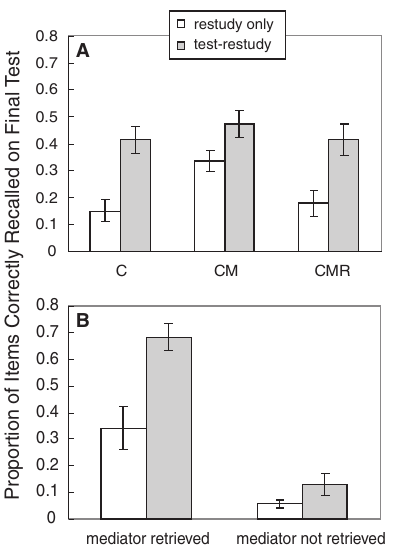
\includegraphics[width=45mm]{figs/l10/pyc_rawson_2010.png}
\end{column}

\begin{column}{70mm}
\begin{itemize}
 \item \textbf{C}ue only
 \item \textbf{C}ue+\textbf{M}ediator generated during learning
 \item Cue+prompt for mediator \textbf{CMR}
 \item<2->[$\rightarrow$] \textbf{C}: basic testing effect
 \item<3->[$\rightarrow$] \textbf{CM}: test-restudy participants generate more effective mediators
 \item<4->[$\rightarrow$] \textbf{CMR}: test-restudy participants perform better at remembering mediators
\end{itemize}
 
\end{column}
\end{columns}

\begin{itemize}
 \item<5->[$\Rightarrow$] retrieval practice allows people to evaluate the effectiveness of their mediators and replace them with more effective ones
\end{itemize}
\end{overlayarea}
\end{frame}


\begin{frame}
 \frametitle{Implicit learning}
\begin{overlayarea}{110mm}{80mm}
 Can you learn something without being aware of it? \vspace{2mm}

\only<2->{
\textbf{Implicit learning} is the process through which we become sensitive to certain regularities in the environment
\begin{enumerate}
 \item<3-> in the \textit{absence of intention} to learn about these regularities
 \item<4-> in the \textit{absence of awareness} that one is learning
 \item<5-> in such a way that the resulting \textit{knowledge is difficult to express}
\end{enumerate}
}

\only<6->{
\textbf{Explicit} vs \textbf{implicit} learning:
\begin{enumerate}
 \item Age independence
 \item IQ independence
 \item Robustness
 \item Low variability
 \item Common to most species
\end{enumerate}
}
\end{overlayarea}
\end{frame}



\begin{frame}
 \frametitle{How to assess implicit learning}
\begin{overlayarea}{110mm}{60mm}
\textbf{Serial reaction time task}
\begin{itemize}
 \item on each trial a stimulus appears at one of several different locations on the screen
 \item participants respond rapidly by pressing the key corresponding to its location
 \item some sequences are repeated throughout the experiment
 \item[$\Rightarrow$] participants responses are faster to repeated than to novel sequences
\end{itemize}
\end{overlayarea}
\end{frame}




\begin{frame}
 \frametitle{How to assess implicit learning}
\begin{overlayarea}{110mm}{80mm}

Haider et al., 2011
\only<1>{
\begin{itemize}
 \item \textit{Press the square that corresponds to the colour word!}
 \item congruent and incongruent trials
 \item over each set of six trials the correct coloured square followed a regular sequence (1-6-4-2-3-5) unbeknownst to the participants
\end{itemize}
}

\begin{center}
\includegraphics<1>[width=40mm]{figs/l10/haider_2011_stimulus.png}
\includegraphics<2->[width=80mm]{figs/l10/haider_2011_RT_drop.png}
\end{center}

\only<2->{
\begin{itemize}
 \item 91\% of the RT-drop participants (34\%) correctly described the training sequence compared to 0\% of the no-RT-drop group
\end{itemize}
}
\end{overlayarea}
\end{frame}



\begin{frame}
 \frametitle{Implicit learning in the real world}
\begin{overlayarea}{110mm}{75mm}
 Snyder et al., 2014: Typing skill in college students
\begin{itemize}
 \item \textit{Write the letters in their correct locations!}
 \item<2-> 15 of the letters (60\%) were located correctly (correct, omit, misplaced)
\end{itemize}
\begin{center}
\includegraphics<1>[width=80mm]{figs/l10/snyder_2013_keyboard.png}
\includegraphics<2->[width=80mm]{figs/l10/snyder_2013_results.png}
\end{center}

\begin{itemize}
 \item<3->[!] Accurate identification due to explicit memory or simulated typing?
 \item<4-> performance was significantly reduced in a motor suppression condition
\end{itemize}
\end{overlayarea}
\end{frame}


\begin{frame}
 \frametitle{Summary: Implicit learning}

\begin{overlayarea}{110mm}{60mm}
 
\begin{itemize}
\setlength{\itemsep}{6pt}
 \item implicit and explicit learning partially follow different rules
 \item initial explicit learning might lead to implicit memory
 \item explicit and implicit memory system are likely to interact in ways that are still not understood 
\end{itemize}
\end{overlayarea}
\end{frame}


\begin{frame}
 \frametitle{Forgetting}
\begin{overlayarea}{110mm}{70mm}
 Ebbinghaus, 1885: \textbf{Savings method}

\begin{itemize}
 \item he (!) learned lists of nonsense syllables until he recalled 100\%
 \item his basic measure of forgetting was the time required to reach the original learning state, \# trials
 \item measured the amount of saving after different time intervals
\end{itemize}

\begin{columns}[T]
\begin{column}{50mm}
\includegraphics<1>[width=60mm]{figs/l10/ebbinghaus_forgetting.png}
\end{column}

\begin{column}{40mm}
\begin{center}
\begin{itemize}
 \item[!] most rapid forgetting over the first hour 
\end{itemize}
\end{center}
\end{column}
\end{columns}

\end{overlayarea}
\end{frame}


\begin{frame}
 \frametitle{Forgetting from long-term memory}
\begin{overlayarea}{110mm}{80mm}
\textbf{Decay}
 \begin{itemize}
  \setlength{\itemsep}{2pt}
  \item forgetting due to gradual loss of the substrate of memory
  \item we form numerous trivial memories each day 
  \item[$\rightarrow$] active removal process
 \end{itemize}
 \only<2->{
\textbf{Interference}
  \begin{itemize}
  \setlength{\itemsep}{2pt}
  \item proactive - disruption of memory by previous learning
  \item<3-> retroactive - disruption of memory for what was previously learned by other learning during retention interval
 \end{itemize}
}
\centering
\includegraphics<4>[width=60mm]{figs/l10/interference.png}
\end{overlayarea}
\end{frame}

\begin{frame}
 \frametitle{Forgetting: proactive interference}
\begin{overlayarea}{110mm}{80mm}
 B\"auml and Kliegl, 2013
\begin{itemize}
 \item hypothesis: proactive interference because memory search is too broad including irrelevant material
 \item<2-> test: learning of word lists in one of three conditions
 \begin{itemize}
  \item \textbf{R}emember condition: 3 lists were learned, free recall of last list
  \item \textbf{F}orget condition: participants were told after learning of the first two lists to forget them, free recall of the last list
 \item \textbf{C}ontrol condition: learning and testing only on last list 
 \end{itemize}
 \item<3-> results: \textbf{C} - 68\% vs. \textbf{R} - 41\% correct, \only<4->{\textcolor{blue}{\textbf{F} - 68\% correct}}
\item[]
\item<5-> anecdotal evidence suggests that people adopt active strategies to minimize interference also in real life
\end{itemize}
\end{overlayarea}
\end{frame}

\begin{frame}
 \frametitle{Cue-dependent forgetting}
\begin{overlayarea}{110mm}{80mm}
 Tulving, 1979: \textbf{The encoding specificity principle}
\begin{itemize}
 \item forgetting occurs when there is a poor match between information in the memory trace and information at retrieval
 \item importance of context: external and internal (mood-state-dependent memory)
\end{itemize}
\only<2->{
Godden and Baddeley, 1980
 
\centering
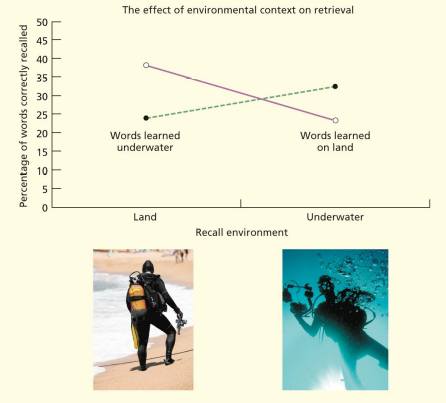
\includegraphics[width=50mm]{figs/l10/context_learning.png}
}
\end{overlayarea}
\end{frame} 



\begin{frame}
 \frametitle{Summary}
\begin{itemize}[<+->]
\setlength{\itemsep}{2pt}
 \item according to the \textbf{multi-store model} there are separate stores for holding sensory, short-term and long-term information, supported by lesion studies but oversimplification

 \item \textbf{WM model} consists of: central executive, phonological loop, visuo-spatial sketchpad, episodic buffer, central executive used for executive functions such as inhibition, shifting and updating of WM content

 \item \textbf{WM capacity} correlates with other cognitive measures such as attentional control, fluid intelligence, planning, ...

 \item LTM is better when the learning period includes \textbf{retrieval practice} in addition to study, retrieval practice might improve retrieval mediators

 \item behavioral findings support the distinction between \textbf{implicit and explicit learning} but they are likely to interact
 
 \item proactive and retroactive interference are responsible for \textbf{forgetting}, people can use strategies to minimise proactive interference 
\end{itemize}
\end{frame}



\begin{frame}
 \frametitle{References}
\begin{small}
\begin{itemize}
 \item  Eysenck, M. W. \& Keane, M.T. (2015). \textit{Cognitive Psychology. A student's handbook}. Psychology Press: Hove, East Sussex. 
\end{itemize}
\end{small}
\end{frame}


\end{document}